%% jan. 4, 2011  items to fix:
%% notation for math and reference to images.
%% how include eps figures.
%% make all the little figures (search for eps) in a common, nice matlab way for the
%% example filtering operations.

%\chapter{Filter jets, scales and orientations}
\chapter{Filter Banks}
\label{chapter:filter_banks}

\section{Introduction}

Although linear filters can perform a wide range of operations as we have seen in previous chapters, image understanding requires nonlinear operators. In this chapter we will study how sets of filters can be used to extract information about images. We will focus on some traditional families of filters that have been used to build image representations in the early days of computer vision and that help to understand part of the representational power of modern deep neural networks.

We will show how simple nonlinearities applied to the output of linear filters (such as the squaring nonlinearity) can be used to build useful image representations.

% All the filters we have seen until here are linear. Introducing non-linearities 

\section{Gabor Filters}
\index{Filter!Gabor filter}

In \chap{\ref{chapter:fourier_analysis}} we discussed several useful image representations: representing an image in the frequency domain and decomposing it into amplitude and phase, and also the analysis of image content across different scales and orientations. The Fourier transform is a tool that allows us to extract that information, but only globally. For this information to be useful it needs to be localized. For instance, the analysis of orientations of local image structures can be done using image gradients (\chap{\ref{chapter:image_derivatives}}), which are localized in space. In fact, we made use of image derivatives in \chap{\ref{chapter:simplesystem}} to recover the three-dimensional (3D) structure of a scene. Here we will discuss another family of filters that has a long history of being used for image analysis: Gabor filters.

%Gabor filters allow analyzing the local frequency content (amplitude and phase). 



\Fig{\ref{fig:1D_gabor_function}}{a} shows a one-dimensional (1D) sine function. This function has infinite support. When used as a representation, the Fourier coefficients are obtained as the scalar product between the sine wave and the input image. Each Fourier coefficient involves a point-wise multiplication between the wave and the input image and then the sum of the result. As a consequence of the infinite support of the wave, one single Fourier coefficient does not tell us anything about what happens locally inside the analyzed image.

A good start for a localized image analysis is to restrict the spatial support of a sinusoidal basis function. One function that has a local support (a lots of nice properties as we discussed in \chap{\ref{chap:blur_filters}}) is the Gaussian function (\fig{\ref{fig:1D_gabor_function}}[b]). The product of the Gaussian and the sine wave (or a cosine wave) gives the function with the profile shown in \fig{\ref{fig:1D_gabor_function}}{c} called a Gabor filter. Gabor functions were introduced by Dennis Gabor in 1946 \cite{Gabor1946TheoryOC}.


\begin{figure}
	\centerline{
		\sublabel{a}{
			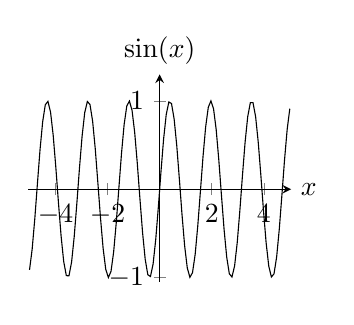
\begin{tikzpicture}
				\begin{axis} [width=140pt,height=120pt,
						axis x line=middle,
						axis y line=middle,
						tick align=center,
						every axis x label/.style={at={(current axis.right of origin)},anchor=west},
						every axis y label/.style={at={(current axis.above origin)}, anchor=north east,above=0mm},
						xmin=-5.05, xmax=5.05,
						xtick={-4,-2,0,2,4},
						xlabel=$x$,
						ymin=-1.05, ymax=1.3,
						ytick={-1,0,1},
						ylabel={$\sin(x)$},
						color=black]
					\addplot[domain=-5:5,samples=100,samples y=0]
					({x}, {sin(deg(4*x))});
				\end{axis}
			\end{tikzpicture}
		}
		\sublabel{b}{
			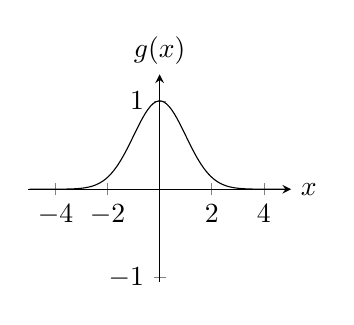
\begin{tikzpicture}
				\begin{axis} [width=140pt,height=120pt,
						axis x line=middle,
						axis y line=middle,
						tick align=center,
						every axis x label/.style={at={(current axis.right of origin)},anchor=west},
						every axis y label/.style={at={(current axis.above origin)}, anchor=north east,above=0mm},
						xmin=-5.05, xmax=5.05,
						xtick={-4,-2,0,2,4},
						xlabel=$x$,
						ymin=-1.05, ymax=1.3,
						ytick={-1,0,1},
						ylabel={$g(x)$},
						color=black]
					\addplot[domain=-5:5,samples=100,samples y=0]
					({x}, {exp(-(x^2)/2)});
				\end{axis}
			\end{tikzpicture}
		}
		\sublabel{c}{
			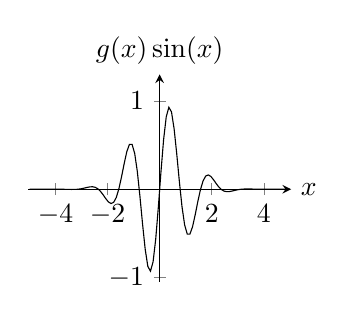
\begin{tikzpicture}
				\begin{axis} [width=140pt,height=120pt,
						axis x line=middle,
						axis y line=middle,
						tick align=center,
						every axis x label/.style={at={(current axis.right of origin)},anchor=west},
						every axis y label/.style={at={(current axis.above origin)}, anchor=north east,above=0mm},
						xmin=-5.05, xmax=5.05,
						xtick={-4,-2,0,2,4},
						xlabel=$x$,
						ymin=-1.05, ymax=1.3,
						ytick={-1,0,1},
						ylabel={$g(x)\sin(x)$},
						color=black]
					\addplot[domain=-5:5,samples=100,samples y=0]
					({x}, {exp(-(x^2)/2)*sin(deg(4*x))});
				\end{axis}
			\end{tikzpicture}
		}
	}
	\caption{Construction of a Gabor function. (a) Sine function. (b) Gaussian function. (c) Gabor function obtained as the product of (a) and (b).}
	\label{fig:1D_gabor_function}
\end{figure}



Gabor functions, originally proposed in 1D, were made popular as an operator for image analysis by Goesta Granlund in his paper \booktitle{In Search of a General Picture Processing Operator} \cite{GRANLUND1978155}.
\marginnote{Gabor functions are localized in both the spatial and frequency domain. One remarkable property of the Gabor function is that it is the optimal function that achieves the best simultaneous localization in space and frequency.}

Gabor functions can be extended to two dimensions by using 2D Gaussians and waves. We can also use complex waves (\chap{\ref{chapter:fourier_analysis}}) as they will give us a more general form of the Gabor function. We can  multiply a complex Fourier basis function, $\exp{ \left(j  \left(u_0 x + v_0 y \right)  \right)}$,  by a spatially localized 2D Gaussian window, $\exp{\left(-\frac{x^2 + y^2}{2 \sigma^2} \right) }$ to obtain a Gabor function,
$\psi(x,y)$:
\begin{equation}
	\psi(x,y;u_0,v_0) = \frac{1}{2\pi \sigma^2} \exp{\left(-\frac{x^2 + y^2}{2 \sigma^2} \right)} \exp{ \left( j \left(u_0 x + v_0 y \right) \right)}
	\label{eq:gaborcomplexfilter}
\end{equation}

A Gabor function defined as in \eqn{\ref{eq:gaborcomplexfilter}} is a complex-valued function of location and frequency. We can get the cosine and sine waves by looking at the real and imaginary components, $\psi(x,y;u_0,v_0) =  \psi_r(x,y;u_0,v_0) + j \psi_i(x,y;u_0,v_0)$ with
\begin{equation}
	\psi_r(x,y;u_0,v_0) = \frac{1}{2\pi \sigma^2} \exp{\left(-\frac{x^2 + y^2}{2 \sigma^2} \right)} \cos{ \left(u_0 x + v_0 y \right) }
\end{equation}
\begin{equation}
	\psi_i(x,y;u_0,v_0) = \frac{1}{2\pi \sigma^2} \exp{\left(-\frac{x^2 + y^2}{2 \sigma^2} \right)} \sin{ \left(u_0 x + v_0 y \right) }
\end{equation}
Where $\psi_r(x,y;u_0,v_0)$ and $\psi_i(x,y;u_0,v_0)$ are the cosine and sine phase Gabor filters. \Fig{\ref{fig:gabors}} shows the Gaussian window and the real and imaginary parts of the Gabor function.


%\begin{figure}
%\centerline{
%\includegraphics[width=0.8\linewidth]{figures/figs3/gabors.pdf}
%}
%\caption{
%Gabor functions.  Left column:  The localizing Gaussian
%  window, which can be thought of as a Gabor function for a zero
%  frequency sinusoid.  Middle 
%and left columns:  cosine (top row) and sine (bottom row) phase Gabor
%functions for spatial frequencies $u_0 = 0.1$ (middle column) and 
%$u_0 = 0.2$ (right column).  Note the spatial localization of the
%sinusoids, modulated by a Gaussian function of standard deviation
%$\sigma$.  These functions are also localized in spatial frequency
%(not shown), blurred from delta functions in frequency by a Gaussian
%function of  of standard deviation 
%$\frac{1}{\sigma}$.
%} 
%\label{fig:gabors}
%\end{figure}
%
%




\begin{comment}

\begin{figure}
	%\centerline{
	\sublabel{a}{
	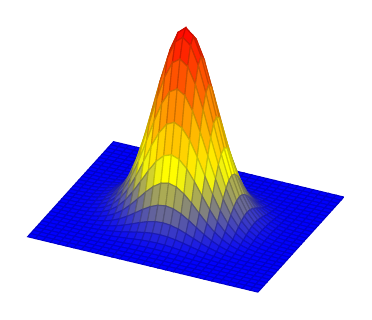
\begin{tikzpicture}
		\begin{axis}
			[width=167pt,height=190pt,
				xmin=-4, xmax=4,
				xlabel={$x$},
				ymin=-6, ymax=4,
				ylabel={$y$},
				hide axis,
				colormap/hot]
			\addplot3[domain=-4:4,samples=31,surf] {1/(2*pi)*exp(-(x^2+y^2)/2)};
			%\node at (0,-5) {(a)};
		\end{axis}
	\end{tikzpicture}
	%}
	\sublabel{b}{
		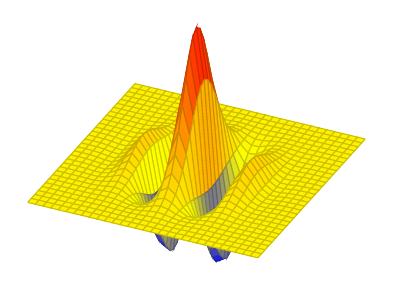
\begin{tikzpicture}
			\begin{axis}
				[width=167pt,height=190pt,
					xmin=-4, xmax=4,
					%xtick={-3, -1, 0, 1, 3},
					xlabel=$x$,
					ymin=-4, ymax=4,
					%ytick={-1,0,1},
					ylabel={$y$},
					hide axis,
					axis lines = left,
					colormap/hot]
				\addplot3[domain=-4:4,samples=31,surf]
				{1/(2*pi)*exp(-(x^2+y^2)/2)*cos(deg(2*pi*x/4*2))};
				%{cos(deg(2*pi*x/4*1))};
				%\node at (0,-1) {(b)};
			\end{axis}
		\end{tikzpicture}
	}
	\sublabel{c}{
	\begin{tikzpicture}
		\begin{axis}
			[width=167pt,height=190pt,
				xmin=-4, xmax=4,
				%xtick={-3, -1, 0, 1, 3},
				xlabel=$x$,
				ymin=-4, ymax=4,
				%ytick={-1,0,1},
				ylabel={$y$},
				hide axis,
				axis lines = left,
				colormap/hot]
			\addplot3[domain=-4:4,samples=31,surf]
			{1/(2*pi)*exp(-(x^2+y^2)/2)*sin(deg(2*pi*x/4*2))};
			%\node at (0,-1) {(c)};
			%{sin(16*2*pi*x)};
			}
		\end{axis}
	\end{tikzpicture}
	%}
	\caption{2D Gabor functions.  (a) The localizing Gaussian window ($\sigma=1$), which can be thought of as a Gabor function for a zero frequency sinusoid.  (b) Cosine, and (c) sine phase Gabor functions with central frequency $u_0=2\pi$ and $v_0=0$.}
	\label{fig:gabors}
\end{figure}

\end{comment}



\begin{figure}
	\centerline{
		(a)
		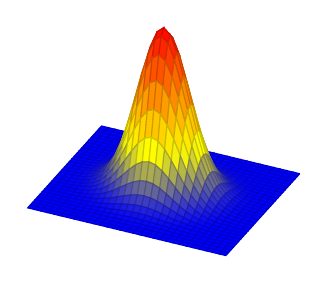
\begin{tikzpicture}
			\begin{axis}
				[width=150pt,height=170pt,
					xmin=-4, xmax=4,
					xlabel={$x$},
					ymin=-6, ymax=4,
					ylabel={$y$},
					hide axis,
					colormap/hot]
				\addplot3[domain=-4:4,samples=31,surf] {1/(2*pi)*exp(-(x^2+y^2)/2)};
			\end{axis}
		\end{tikzpicture}
		~(b)
		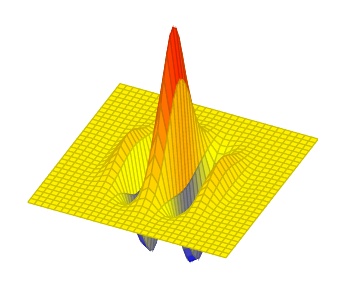
\begin{tikzpicture}
			\begin{axis}
				[width=150pt,height=190pt,
					xmin=-4, xmax=4,
					%xtick={-3, -1, 0, 1, 3},
					xlabel=$x$,
					ymin=-4, ymax=4,
					%ytick={-1,0,1},
					ylabel={$y$},
					hide axis,
					axis lines = left,
					colormap/hot]
				\addplot3[domain=-4:4,samples=31,surf]
				{1/(2*pi)*exp(-(x^2+y^2)/2)*cos(deg(2*pi*x/4*2))};
			\end{axis}
		\end{tikzpicture}
		~(c)
		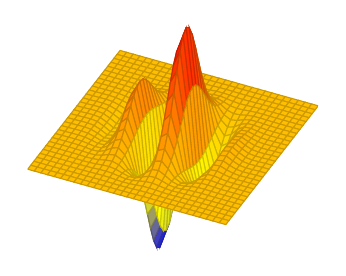
\begin{tikzpicture}
			\begin{axis}
				[width=150pt,height=190pt,
					xmin=-4, xmax=4,
					%xtick={-3, -1, 0, 1, 3},
					xlabel=$x$,
					ymin=-4, ymax=4,
					%ytick={-1,0,1},
					ylabel={$y$},
					hide axis,
					axis lines = left,
					colormap/hot]
				\addplot3[domain=-4:4,samples=31,surf]
				{1/(2*pi)*exp(-(x^2+y^2)/2)*sin(deg(2*pi*x/4*2))};
			\end{axis}
		\end{tikzpicture}
	}
	\caption{2D Gabor functions.  (a) The localizing Gaussian window ($\sigma=1$), which can be thought of as a Gabor function for a zero frequency sinusoid.  (b) Cosine, and (c) sine phase Gabor functions with central frequency $u_0=2\pi$ and $v_0=0$.}
	\label{fig:gabors}
\end{figure}

The Fourier transform of a complex Gabor function is a Gaussian in the Fourier domain shifted with respect to the origin:
%\begin{equation}
%\Psi(u,v;u_0,v_0) =\exp{\left(-2 \pi^2 \left((u-u_0)^2 + (v-v_0)^2 \right) \sigma^2 \right)} 
%\end{equation}
\begin{equation}
	%\Psi(u,v; u_0,v_0) = \exp{ \left( -\frac{\left((u-u_0)^2 + (v-v_0)^2 \right) \sigma^2}{2} \right) } 
	\Psi(u,v; u_0,v_0) = \exp{ \left( -  \left((u-u_0)^2 + (v-v_0)^2 \right) \frac{\sigma^2}{2} \right) }
\end{equation}

\marginnote{The Gabor filter is an oriented band-pass filter.}

\Fig{\ref{fig:gabor_ft}} shows the magnitude of the Fourier transform of the Gabor filters.  \Fig{\ref{fig:gabor_ft}}{a} shows the cosine phase Gabor function, $\psi_r(x,y;u_0,v_0)$, and \fig{\ref{fig:gabor_ft}}{b} shows the sine phase Gabor function, $\psi_i(x,y;u_0,v_0)$. \Fig{\ref{fig:gabor_ft}}{c} shows the Fourier transform of the cosine phase Gabor function, $\Psi_r(u,v;u_0,v_0)$, and \fig{\ref{fig:gabor_ft}}{d} shows the Fourier transform of the complex Gabor function, $\Psi(u,v;u_0,v_0)$.

\begin{figure}
	\centerline{
		\includegraphics[width=1\linewidth]{figures/spatial_filter_sets/gabor_FT.eps} }
	\caption{(a) Cosine and (b) sine Gabor functions. (c) Magnitude of the Fourier transform of both the cosine and sine Gabor functions (their FT only differs in the phase). (d) FT of the complex Gabor function, which is asymmetrical with a single lobe.}
	\label{fig:gabor_ft}
\end{figure}
%\vspace{-.2in}

\Fig{\ref{fig:gabor_ex_ft}} shows how the Gabor function changes when modifying its parameters (central frequency, $(u_0,v_0)$, and width, $\sigma$).
The value of $\sigma$ sets the locality of the window of analysis and the values of $(u_0,v_0)$ adjust the orientation of the Gabor function and frequency.  A large $\sigma$ makes the spatial extend large and the frequency extend small.  A small value of $\sigma$ has the opposite behavior.
Analyzing the image with a set of Gabor functions with a large $\sigma$ is like computing the Fourier transform of the image.

%%%%The central frequency changes the orientation and the scale at which the filter is most sensitive for, and the sigma changes the spatial and the frequency extend of the signal. A large $\sigma$ makes the spatial extend large and the frequency extend small.  A small value of $\sigma$ has the opposite behavior. 

\begin{figure}
	\centerline{
		\includegraphics[width=1\linewidth]{figures/spatial_filter_sets/gabor_examples_FT.eps} }
	\caption{Cosine phase Gabor functions tuned to different widths, frequencies, and orientations, and their corresponding Fourier transforms (only the magnitude is shown).}
	\label{fig:gabor_ex_ft}
\end{figure}


The sine phase Gabor function is zero mean. However, the cosine phase Gabor function is not zero mean. The Gaussian width $\sigma$ has to be sufficiently large so that the Gabor function behaves like a zero mean filter. All the previous definitions are given in the continuous domain. The discrete version of the Gabor function is obtained by sampling the continuous functions.

One important characteristic of Gabor filters is that they are very similar to the shape of some cortical receptive fields found in the mammalian visual system. This provides a hint that we're on the right track with these filters to build image representations.

\marginnote{Remember the description of simple and complex cells in the visual system from \chap{\ref{chap:challenge_of_vision}}.}


The convolution of the Gabor function with an image, $\img (x,y)$ results in an output image that depends on both space, $(x,y)$, and frequency, $(u,v)$:
\begin{equation}
	\label{eq:gaborconv}
	\img_{\psi} \left(x,y,u,v \right) = \img \left(x,y\right) \circ \psi(x,y;u,v)
\end{equation}


\Fig{\ref{fig:gabor_zebra}} shows the result of the convolution between a picture and the cosine and sine phase Gabor functions at three different scales ($\sigma = 2,4,8$). In this example, the Gabor filters are tuned to detect vertical edges. Gabor filters are useful for analyzing line or edge phase structures in images.  But they have many other benefits when we combine them together in quadrature pairs.


\begin{figure}[t]
	\includegraphics[width=1\linewidth]{figures/spatial_filter_sets/gabor_zebra.eps}
	\caption{Zebra picture filtered by cosine and sine Gabor functions at three scales with $\sigma = 2,4,8$ and $u_0 = 1/(2\sigma)$, $v_0=0$. Each row shows one scale. (a) Cosine and sine Gabor filters. (b) Cosine and sine outputs. (c) Magnitude and phase of the output of the complex Gabor filter.}
	\label{fig:gabor_zebra}
\end{figure}

\subsection{Quadrature Pairs and the Hilbert Transform}

Pairs of filters can be in a relationship to each other that is called {\bf quadrature phase}.
\index{Filter!Quadrature phase}
This relationship is useful for many low-level visual processing tasks.  When in quadrature phase, pairs of oriented filters can measure what is called local oriented energy, can identify contours, independently of the phase of the contour, and can measure positional changes very accurately. Let's start with the mathematical definition of quadrature.

% is the fact that the energy response to the line signal is
% wider than the energy response to the edge signal significant?  I
% don't think so and I should remake these images to be sure it's not
% simply some artifact of how it was processed.

For notational simplicity, we'll describe quadrature pair filters in the time domain, but they extend naturally to two or more dimensions. Consider an even symmetric zero-mean signal, $\img (t)$, and with Fourier transform $\capitalimg (\omega)$, with $\capitalimg(0)=0$ because the signal is zero-mean. In the Fourier domain, two functions, $\capitalimg (\omega)$ and $\capitalimg_h(\omega)$, are said to be Hilbert transform pairs if:
\begin{equation}
	\capitalimg_h(\omega) = \begin{cases}
		~  - j \capitalimg(\omega) & \quad \text{if } \omega >0 \\
		j \capitalimg(\omega)      & \quad \text{if } \omega <0 \\
	\end{cases}
\end{equation}

We now define the complex signal:
\begin{equation}
	\img_a(t) = \img(t) + j \img_h(t)
	\label{eq:analyticsignal}
\end{equation}
where $\img_h(t)$ is the Hilbert transform of $\img(t)$.
The signal $\img_a(t)$ is called the {\bf analytic signal}
\index{Signals!Analytic signal}
and its Fourier transform has no negative frequency components. It is easy to show that
\begin{equation}
	\capitalimg_a(\omega) = \begin{cases}
		~  2\capitalimg(\omega) & \quad \text{if } \omega >0 \\
		0                       & \quad \text{if } \omega <0 \\
	\end{cases}
\end{equation}
It is interesting to write the complex signal $\img_a(t)$ in polar form:
\begin{equation}
	\img_a(t) = a(t) \exp \left( j \, \theta (t) \right)
	\label{eq:analyticsignalpolar}
\end{equation}
where $a(t)$ is the instantaneous amplitude ({\bf local amplitude})
and $\theta (t)$ is the instantaneous phase ({\bf local phase}).
This particular representation is common in communications theory, and it has been used to build image representations invariant to certain image structures as we will discuss in the following sections.

The extension of the Hilbert transform to images can be done in several ways. The most common approach in image processing is to define one direction in the frequency space $n$ and then the Hilbert transform is as follows:
\begin{equation}
	\capitalimg_h(\omega_x,\omega_y) = \begin{cases}
		~  - j \capitalimg(\omega_x,\omega_y) & \quad \text{if } n^T \cdot (\omega_x,\omega_y) > 0 \\
		j \capitalimg(\omega_x,\omega_y)      & \quad \text{if } n^T \cdot (\omega_x,\omega_y) <0  \\
	\end{cases}
\end{equation}

Two band-pass filters are said to be in quadrature if the impulse responses are Hilbert transform pairs along some orientation in the frequency domain.  Sine and cosine functions of the same frequency are Hilbert transform pairs, as are sine and cosine phase Gabor functions, of the same frequency and Gaussian envelope parameters.  Thus, these filter pairs are also quadrature pairs. When convolving two filters in quadrature with a signal (or image) the two outputs are also in quadrature.

The quadrature in the Gabor functions is an approximation that only holds for $\sigma$ sufficiently large. For small $\sigma$ the filter does not form a quadrature pair. For large $\sigma$, the real and imaginary parts of the Gabor filter (cosine and sine phase local filters) are filters in quadrature with the vector $n=(u_0,v_0)$ pointing in the direction of the central frequency of the Gabor function.

\subsection{Local Amplitude}

Let $h(x,y)$ and $q(x,y)$ be band-pass filters in quadrature, and let $\img_h(x,y)$ and $\img_q(x,y)$ be the result of convolving the signal $\img(x,y)$ with $h(x,y)$ and $q(x,y)$, respectively.  Then, the squared local amplitude is a measure of the image power within the frequency bandwidth of the filters in the local neighborhood of $(x,y)$:
\begin{equation}
	a^2(x,y) = \img_h(x,y)^2 + \img_q(x,y)^2
\end{equation}
\Fig{\ref{fig:quad2}} shows the steps to compute the local amplitude of an input image using Gabor filters. This is like a two-layer convolutional neural network with two channels in the first layer, a squaring nonlinearity and then followed by a sum in the second layer. This very simple system can perform a number of interesting operations.

\begin{figure}[t]
	\centerline{
		\includegraphics[width=0.5\linewidth]{figures/spatial_filter_sets/gabor_magnitude.eps}}
	\caption{Computation of localized amplitude. The input is filtered by a pair of quadrature Gabor filters. Each filter output is squared and the result is added.}
	\label{fig:quad2}
\end{figure}

To see how useful the local amplitude is, let's start by computing it for some simple images. If the input image is a delta, $\img(x,y) = \delta(x,y)$ (this is an image with a single bright dot on it), and the filters $h$ and $q$ are the cosine and sine phase Gabor filters, then, the local amplitude image is:
\begin{equation}
	\begin{split}
		a(x,y) & = \sqrt{\img_h(x,y)^2 + \img_q(x,y)^2} =                                    \\
		       & = \sqrt{\psi^2_r(x,y;u_0,v_0) + \psi^2_i(x,y;u_0,v_0)} =                    \\
		       & = \frac{1}{2\pi \sigma^2} \exp{\left(-\frac{x^2 + y^2}{2 \sigma^2} \right)}
	\end{split}
\end{equation}
The amplitude of the delta function is the Gaussian envelope of the Gabor function. This result is independent of the contrast of the input image. For instance, if the input is $\img(x,y) = -\delta(x,y)$, the amplitude image does not change (it is {\bf sign invariant}). \Fig{\ref{fig:quad3}}{a} shows an image with two impulses of opposite signs. \Fig{\ref{fig:quad3}}{b} show the output of the cosine and sine filters, and \fig{\ref{fig:quad3}}{c} shows the local amplitude $a(x,y)$. The local amplitude is two Gaussians centered on each impulse. Note that the sign of each impulse does not affect the sign or shape of the local amplitude. Therefore, this system is sign invariant.

The sign invariance property is specially useful when using the local amplitude to localize edges in images.  \Fig{\ref{fig:quad3}}{d} shows an image composed of several squares. Each square is defined by different polarities with respect to the background. Two of the squares are solid while the other two are only defined by lines. The local amplitude, \fig{\ref{fig:quad3}}{f}, provides a detector for the square boundaries that is invariant to all those changes. The differences between all the squares are encoded in the local phase image as we will discuss in the following section. \Fig{\ref{fig:gabor_zebra}} shows the local amplitude signal computed on real images.




\begin{figure}[t]
	\centerline{
		\includegraphics[width=1\linewidth]{figures/spatial_filter_sets/gabor_quad_examples.eps}
	}
	\caption{Examples of Gabor outputs to illustrate the contrast invariances present in the local amplitude. In these examples the Gabor filters are centered along the horizontal frequency axis ($v_0=0$) therefore detecting only vertical edges.}
	\label{fig:quad3}
\end{figure}




One property to notice in all these examples, is that, although the images $\img_h(x,y)$ and $\img_q(x,y)$ are band-pass, the amplitude $a^2(x,y)$ is a low-pass image. %To check this it is interesting to compute the Fourier transform of $a^2(x,y)$. 
%
%Consider the bandpass filter, $f(x,y)$, with Fourier transform $\mathrm{F}(u,v)$. 
%We can write $\mathrm{F}(u,v)$ as the sum of two functions $\mathrm{F}^{+}(u,v)$ and $\mathrm{F}^{-}(u,v)$ so that $\mathrm{F}^{+}(u,v)=0$ for $n^T \cdot (\omega_x,\omega_y)<0$ and $\mathrm{F}^{-}(u,v)=0$ for $n^T \cdot (\omega_x,\omega_y)>0$. If $f(x,y)$ is even symmetric then we have that $\mathrm{F}^{+}(u,v) = \mathrm{F}^{-}(-u,-v)$, for instance the cosine phase Gabor filter. This decomposition is illustrated in figure~\ref{fig:quad_amplitude_spectrum}.a.
%If the Fourier transform of $I_f(x,y)$ is $\mathrm{I}_f(u,v)$, then the Fourier transform of $I^2_f(x,y)$ is $\mathrm{I}_f(u,v) \circ \mathrm{I}_f(u,v)$. 
%Then the Fourier transform of $I^2_f(x,y)$ is:
%%\begin{equation}
%%\begin{split}
%%\mathrm{I}_f \circ \mathrm{I}_f & =  \left(\mathrm{I}  \mathrm{F} \right) \circ \left(\mathrm{I}  \mathrm{F} \right) = \\
%%& =  \mathrm{I} (\mathrm{F}^+ + \mathrm{F}^-) \circ \mathrm{I} (\mathrm{F}^+ + \mathrm{F}^-) = \\
%%& =  \mathrm{I} \mathrm{F}^+ \circ \mathrm{I} \mathrm{F}^+  + \mathrm{I} \mathrm{F}^- \circ \mathrm{I} \mathrm{F}^- 
%%+  2 \mathrm{I} \mathrm{F}^+ \circ \mathrm{I}  \mathrm{F}^- 
%%\end{split}
%%\end{equation}
%\begin{equation}
%\mathrm{I}_f \circ \mathrm{I}_f =  \mathrm{I} (\mathrm{F}^+ + \mathrm{F}^-) \circ \mathrm{I} (\mathrm{F}^+ + \mathrm{F}^-) =  \mathrm{I} \mathrm{F}^+ \circ \mathrm{I} \mathrm{F}^+  + \mathrm{I} \mathrm{F}^- \circ \mathrm{I} \mathrm{F}^- 
%+  2 \mathrm{I} \mathrm{F}^+ \circ \mathrm{I}  \mathrm{F}^- 
%\end{equation}
%If $h(x,y)$ is the Hilbert transform of $f(x,y)$, then $\mathrm{H}(u,v) = j \left( \mathrm{F}^{+}(u,v) - \mathrm{F}^{-}(u,v) \right)$, as illustrated in figure~\ref{fig:quad_amplitude_spectrum}.b. The Fourier transform of $I^2_h(x,y)$ is:
%%\begin{equation}
%%\begin{split}
%%\mathrm{I}_h \circ \mathrm{I}_h & =  \left(\mathrm{I}  \mathrm{H} \right) \circ \left(\mathrm{I}  \mathrm{H} \right) = \\
%%& =  j\mathrm{I} (\mathrm{F}^+ - \mathrm{F}^-) \circ j\mathrm{I} (\mathrm{F}^+ - \mathrm{F}^-) = \\
%%& =  - \mathrm{I} \mathrm{F}^+ \circ \mathrm{I} \mathrm{F}^+  - \mathrm{I} \mathrm{F}^- \circ \mathrm{I} \mathrm{F}^- 
%%+  2 \mathrm{I} \mathrm{F}^+ \circ \mathrm{I}  \mathrm{F}^- 
%%\end{split}
%%\end{equation}
%\begin{equation}
%\mathrm{I}_h \circ \mathrm{I}_h =  
%%\left(\mathrm{I}  \mathrm{H} \right) \circ \left(\mathrm{I}  \mathrm{H} \right) =  
%j\mathrm{I} (\mathrm{F}^+ - \mathrm{F}^-) \circ j\mathrm{I} (\mathrm{F}^+ - \mathrm{F}^-) =  - \mathrm{I} \mathrm{F}^+ \circ \mathrm{I} \mathrm{F}^+  - \mathrm{I} \mathrm{F}^- \circ \mathrm{I} \mathrm{F}^- 
%+  2 \mathrm{I} \mathrm{F}^+ \circ \mathrm{I}  \mathrm{F}^- 
%\end{equation}
%
%Note that if $\mathrm{I} \mathrm{F}^+$ is centered around the frequency $(u_0,v_0)$, then $\left(\mathrm{I}  \mathrm{F} \right) \circ \left(\mathrm{I}  \mathrm{F} \right)$ is centered around $(2u_0,2v_0)$. Also, $\left(\mathrm{I} \mathrm{F}^+ \right) \circ\left( \mathrm{I}  \mathrm{F}^- \right)$ is centered around the frequency $(0,0)$. This is shown in figures~\ref{fig:quad_amplitude_spectrum}.b and d.
%
%\begin{figure}
%\centerline{
%\includegraphics[width=1\linewidth]{figures/spatial_filter_sets/quad_amplitude_spectrum.eps} 
%}
%\caption{Sketch of the derivation of the Fourier transform of the local amplitude. a) frequency response of even filter $f$, b) a) frequency response of odd filter $h$, c) Fourier transform of $f^2$, d) Fourier transform of $h^2$, e) Fourier transform of $a^2 = f^2+h^2$} 
%\label{fig:quad_amplitude_spectrum}
%\end{figure}
%
%%
%%It is now useful to write $\mathrm{I}_f(u,v)$ as the sum of two components obtained by separating the frequency domain in two half spaces according the the direction $n=(u_0,v_0)$
%%\begin{equation}
%%\mathrm{I}_f(u,v) =  \mathrm{I}^{+}_f(u,v) + \mathrm{I}^{-}_f(u,v)
%%\end{equation}
%%
%%As $\mathrm{I}_f(u,v)$ is the result 
%%\begin{eqnarray} 
%%I_f^2 = \left[I \circ f \right]^2 & \rightarrow^{FT} & 
%%(I  \mathrm{F}) \circ (I F) \\
%%& = & I (F^+ + F^-) \circ I (F^+ + F^-) \\
%%& = & I F^+ \circ I F^+  + I F^- \circ I F^- 
%%+  2 I F^+ \circ I  F^- \\
%%\end{eqnarray} 
%%and, similarly
%%\begin{eqnarray}
%%I_h^2 = \left[ I \circ h \right] ^2 & \rightarrow & 
%%(I  H) \circ (I H) \\
%%& = & j I (F^+ - F^-) \circ j I (F^+ - F^-) \\
%%& = & -I F^+ \circ I F^+  - I F^- \circ I F^- 
%%+  2 I F^+ \circ I  F^- \\
%%\end{eqnarray}
%The Fourier transform of the local amplitude $a^2(x,y) = I_f^2 + I_h^2$ is:%= \left[ I \circ f \right]^2 + \left[I \circ g \right]^2 
%%& \rightarrow & 4 I F^+ \circ I  F^-  %\\
%%& = & \int I(\omega) I(\omega - u) f(\omega) f(\omega - u) d\omega
%\begin{equation}
%%\left(\mathrm{I}  \mathrm{F} \right) \circ \left(\mathrm{I}  \mathrm{F} \right)  + \left(\mathrm{I}  \mathrm{H} \right) \circ \left(\mathrm{I}  \mathrm{H} \right)  
%\mathrm{I}_f \circ \mathrm{I}_f + \mathrm{I}_h \circ \mathrm{I}_h = 4 \mathrm{I} \mathrm{F}^+ \circ \mathrm{I}  \mathrm{F}^-  %\\
%%& = & \int I(\omega) I(\omega - u) f(\omega) f(\omega - u) d\omega
%\label{eq:quadpower}
%\end{equation}
%Eq.~(\ref{eq:quadpower}) reveals that $a^2(x,y)$ is a low-pass signal, as shown shown in figure~\ref{fig:quad_amplitude_spectrum}.e. 
%
%% reveals that the squared sum of the quadrature pair filter responses measures  the square of the Fourier coefficients of $I(\omega)$ within the passband of the filters $f$ and $h$.
%

\subsection{Local Phase}

The local phase is a measure of angle between the real and imaginary components (cosine and sine in the case of complex Gabor filters):
\begin{equation}
	\theta(x,y) = \angle \left[ \img_h(x,y) + j \img_q(x,y) \right]
\end{equation}
where $\theta (x,y)$ is the instantaneous phase (local phase). This is another interesting nonlinearity although it is not commonly used in neural networks. Local image phase has been used to estimate motion \cite{Fleet89}. This information is invariant to local changes of contrast and it is only sensitive to the local image structure.

For oriented, spatial filters, cycling through the phase of the
quadrature pair of filters can generate motion along the direction of
the phase change \cite{Freeman91b}.  %  [[expand on this, show the motion without movement slides.]].






\subsection{Gabor Filter Bank}

Another useful concept is the notion of {\bf filter bank}.
\index{Filter bank}
A filter banks is a collection of filters, each tuned to extract a different image feature, and used to build an image representation.


As shown in \fig{\ref{fig:gabor_ft}}, 2D Gabor filters are selective in spatial frequency. It is very useful to work with sets of Gabor filters, each selective to a different spatial frequency so that they cover the full space of spatial frequencies.

\Fig{\ref{fig:gabor_rectandpolar_tiles}} shows two different arrangements of Gabor filters. \Fig{\ref{fig:gabor_rectandpolar_tiles}}{a} shows a set of Gabor filters sampling the frequency domain using a rectangular grid. \Fig{\ref{fig:gabor_rectandpolar_tiles}}{c} shows the corresponding (cosine) Gabor kernels. All the functions have the same $\sigma$. \Fig{\ref{fig:gabor_rectandpolar_tiles}}{b} shows a polar arrangement of Gabor functions, and \fig{\ref{fig:gabor_rectandpolar_tiles}}{d} the spatial kernels. Here, the Gaussian width $\sigma$ is proportional to the distance between the central frequency and the origin. This produces filters that are rotated and scaled versions of each other.

\begin{figure}[t]
	\centerline{
		\includegraphics[width=1\linewidth]{figures/spatial_filter_sets/gabor_rectandpolar_tiles.eps} }
	\caption{Examples of Gabor sets. Two different ways of tiling the frequency domain.}
	\label{fig:gabor_rectandpolar_tiles}
\end{figure}

If we write in detail the convolution from \eqn{\ref{eq:gaborconv}} we can see that the convolution with a Gabor function is like doing a Fourier transform of the image after applying to it a Gaussian window:
\begin{equation*}
	\begin{split}
		\img_{\psi} \left(x,y,u,v \right) & =   \iint \img \left(x',y'\right) \psi(x-x',y-y';u,v) \, dx' dy' =                                              \\
		                                  & = \iint  \img \left(x',y'\right) g(x-x',y-y') \exp \left( j \left(u (x-x') + v (y-y') \right) \right) dx' dy' = \\
	\end{split}
\end{equation*}
If we extract the term that does not depend on $(x',y')$, and we also use the symmetry of the Gaussian window, we get the following expression:
\begin{equation}
	\begin{split}
		 & = \exp \left( j \left(u x + v y \right) \right) \iint \img \left(x',y'\right) g(x'-x,y'-y) \exp \left(- j \left(u x' + v y' \right) \right) dx' dy'
	\end{split}
\end{equation}
The analogous to the Fourier transform is obtained when we vary the central frequency of the Gabor function $(u,v)$. This is usually called the Gabor transform. Note that the Gabor transform is not self-inverting.



\section{Steerable Filters and Orientation Analysis}


One question that arises with oriented filters is how to change their
orientation.  More precisely, given a filter $h(x,y)$, we want to transform it into a continuous function $h(x,y, \theta)$ of angle $\theta$. The angle $\theta$ specifies the rotation of the original filter $h(x,y)$.

In the case of the Gabor filters, \eqn{\ref{eq:gaborcomplexfilter}}, each orientation requires convolving the image with a Gabor function tuned to that orientation. But do we need to create a new Gabor function for each orientation, or can we interpolate between a fixed number of predefined oriented filter outputs? How many orientations need to be sampled?

\marginnote{In this section we will study a generalization of the Nyquist sampling theorem but applied to dimensions different than space.}


We'd like an analog in orientation for the Nyquist sampling theorem in space:  given a certain number of discrete samples in orientation (or space), can one
interpolate between the samples and synthesize what would
have been found from having a filter (or a spatial sample) at some
arbitrary, intermediate orientation?    The answer is yes, and the
number of filter samples needed to interpolate depends on the form of
the filter.


In \chap{\ref{chapter:image_derivatives}}, we described the simplest example of an oriented filer: a Gaussian derivative. As we discussed in \eqn{\ref{eq:steerable_derivative_filter}}, we can synthesize a directional derivative in
any direction as a linear combination of derivatives in the horizontal
and vertical directions.  By the linearity of convolution, that applies to the derivative
applied to any filter or image, as well. It can be seen that the {\bf steering equation}
\index{Steering equation}
for the first derivative
of a Gaussian filter is
\begin{equation}
	g_{x}(x,y,\theta) = \cos(\theta) g_x(x,y) + \sin(\theta) g_y(x,y)
\end{equation}
where $g_x$ and $g_y$ are the Gaussian derivatives along $x$ and $y$, and $g_{x}(x,y,\theta)$ is the derivative along the direction defined by the angle $\theta$. The interpolation functions are $k_1(\theta) = \cos(\theta)$ and $k_2(\theta) = \sin(\theta)$.

In fact, all higher order Gaussian derivatives have the same property but the number of basis filters changes. For instance, for second-order Gaussian derivatives, the steering equation is:
\begin{equation}
	\begin{split}
		g_{x,x}(x,y,\theta) & = g_{xx}(\cos(\theta) x - \sin (\theta) y, \sin(\theta) x + \cos (\theta)y) =                       \\
		                    & = \cos^2(\theta) g_{xx}(x,y) + \sin^2(\theta) g_{yy}(x,y) - 2 \cos(\theta) \sin(\theta) g_{xy}(x,y)
	\end{split}
\end{equation}
To interpolate the derivative along any orientation requires three basis filters and the interpolation functions are  $k_1(\theta) = \cos^2(\theta)$, $k_2(\theta) = \sin^2(\theta)$, and $k_3(\theta) = -2\cos(\theta)\sin(\theta)$. The minus sign in $k_3$ is due to the positive direction of $\theta$ to be counter-clockwise. \Fig{\ref{fig:steer1}} shows examples for the first- and second-order Gaussian derivatives.

%
%As we know from our 
%differential calculus, we can     On the top row, we see the
%derivative of a Gaussian, horizontal  and vertical,, and one oriented
%at 30 degrees formed as a linear combination of those two.  Again by
%linearity, the output of the 30 filter applied to any image just that
%same linear combination of the outputs of the appropriate basis
%filters applied to those images.



\begin{figure}[h]
	\centerline{
		\includegraphics[width=1\linewidth]{figures/spatial_filter_sets/steer1.eps}
	}
	\caption{The simplest steerable filters: a first-order derivative filter of any
		orientation can be synthesized from a linear combination of two
		basis filter derivatives. The second-order derivative needs three basis.}
	\label{fig:steer1}
\end{figure}



%\begin{figure}
%\centerline{
%\includegraphics[width=0.6\linewidth]{figures/figs3/steerpic.jpg}
%}
%\caption{Example of steering filters using the architecture above.}
%\label{fig:steer2}
%\end{figure}


This leads to an architecture for processing images with oriented {\em steerable} filters shown in \fig{\ref{fig:steer1arc}}. The input images pass through a set of {\bf basis filters},
then the outputs of those filters are modulated with a set of {\bf gain maps}
(which can be different at each pixel).  Those gain maps adjust the
linear combinations of the basis filters to allow the input
filter to be steered to the desired orientations at each position.

\begin{figure}[h]
	\centerline{
		\includegraphics[width=0.6\linewidth]{figures/spatial_filter_sets/steer_architecture.eps}
	}
	\caption{Architecture for steerable filters. This architecture computes the second-order image derivative along orientation $\theta$.}
	\label{fig:steer1arc}
\end{figure}

%In Fig.~\ref{fig:steer2}, we show those basis filters applied to a slightly more interesting image.

In the case of oriented Gabor filters it is not possible to reconstruct exactly any filter orientation by interpolating filter responses. It is interesting to study the conditions in which interpolation gives exact results.

\subsection{Steering Theorem}

Let's make the previous observation more precise and general.  How many basis filters does it take to steer any given
filter?  You could imagine that will depend on how sharply oriented the filter is.  A circularly symmetric filter takes just one basis function
to synthesize all other orientation responses, and a very narrow filter will take quite a few.  This is quantified by steering
theorems.

Let's consider a filter with impulse response $h(x,y)$. For convenience, it is better to write the filter response in polar coordinates, $h(r,\phi)$
The {\bf steering condition} is the requirement that the rotated
filter, $h(r,\phi - \theta)$, be a linear combination of a set of basis filters that are rotated versions of itself, $h(r,\phi - \theta_m)$ with $m \in (1,M)$. The steering condition is:
\begin{equation}
	h(r,\phi - \theta) = \sum_{m=1}^{M} k_{m}(\theta) h(r,\phi - \theta_m) .
	\label{eq:steeringcondition}
\end{equation}

If we express the filter to be steered as a Fourier series in angle (using complex exponentials for notational convenience), we have
\begin{equation}
	h(r,\phi) = \sum_{n=-N}^{N} a_n(r) \exp \left( j n \phi \right)
	\label{eq:fourierseriesinangle}
\end{equation}

Substituting \eqn{\ref{eq:fourierseriesinangle}} into
\eqn{\ref{eq:steeringcondition}}, we have an equation for the
interpolation functions, $k_{j}(\theta)$.
The steering condition, \eqn{\ref{eq:steeringcondition}}, holds for functions
expandable in the form of \eqn{\ref{eq:fourierseriesinangle}} if and only if the
interpolation functions $k_{j}(\theta)$ are solutions of:
%%
\begin{equation}
	\left[
		\begin{array}{c}
			1                 \\
			\exp (j \theta)   \\
			\ldots            \\
			\exp (j N \theta) \\
		\end{array}
		\right]
	=
	\left[
		\begin{array}{cccc}
			1                     & 1                     & \ldots & 1                     \\
			\exp (j \theta_{1})   & \exp (j \theta_{2})   & \ldots & \exp (j \theta_{M})   \\
			\vdots                & \vdots                & \vdots & \vdots                \\
			\exp (j N \theta_{1}) & \exp (j N \theta_{2}) & \ldots & \exp (j N \theta_{M})
		\end{array}
		\right]
	\left[
		\begin{array}{c}
			k_{1}(\theta) \\ k_{2}(\theta) \\ \vdots \\ k_{M}(\theta)
		\end{array}
		\right].
	\label{eq:theorembigmatrix}
\end{equation}

Let's check this for a simple example.  Our derivative of a Gaussian filter (equation [\ref{eq:derivate1gauss2dcont}]) is $x$ times a
Gaussian.  When changing to polar coordinates $x=r \cos( \theta)$, which gives an angular distribution times a radially symmetric Gaussian when written in polar coordinates.  This requires two complex exponentials to write (to create the $\cos (\theta)$ from complex exponentials) and thus requires two basis functions to steer.

Sometimes its more convenient to think of the filters as polynomials times radially symmetric window functions (this is the case for high-order Gaussian derivatives).  Then you can show that for an $N$-th order polynomial with even or odd symmetry $N+1$ basis functions are sufficient \cite{Freeman91}.

Although everything has been derived in the continuous domain, steerability is a property that still holds after sampling the filter function. This is because spatial sampling and steerability are interchangeable: the weighted sum of spatially sampled function is equal to the spatial sampling of the same weighted sum of continuous basis functions.

For computational efficiency, it's more convenient to have the basis filters all be $x-y$ separable functions.  In many cases,
it's straightforward to find such basis functions, and where it's not, there are simple numerical methods to find the best fitting $x-y$
separable basis set.  %See for example \cite{perona}.


\subsection{Steerable Quadrature Pairs}

As in the case of Gabor filters, it is useful to build quadrature pairs of steerable filters. Steerable-quadrature filters allow for arbitrary shifts both in orientation and in phase. We can design such filters. For instance, let's consider the second-order derivatives of a Gaussian with $\sigma^2=1/2$ and normalized so that the integral over all the space of its squared magnitude equals 1:
\begin{equation}
	\begin{split}
		g_{xx}(x,y) & = 0.9213(2x^2-1) \exp \left(-(x^2+y^2) \right) \\
		g_{xy}(x,y) & = 1.843 (x y) \exp \left(-(x^2+y^2) \right)    \\
		g_{yy}(x,y) & = 0.9213(2y^2-1) \exp \left(-(x^2+y^2) \right)
	\end{split}
\end{equation}
It is possible to get a good approximation to its Hilbert transform using a Gaussian times a third-order odd polynomial. The approximation to the Hilbert transform of $g_{xx}(x,y)$ is:
\begin{equation}
	h_{xx}(x,y) = -0.9780 (-2.254 x+x^3) \exp \left(-(x^2+y^2) \right)
\end{equation}
where $g_{xx}(x,y)$ and its Hilbert transform $h_{xx}(x,y)$ have the same spectral content, but the opposite phase. \Fig{\ref{fig:steerg2h2}} analyzes the quality of the approximation. The figure shows the quadrature pair, $g_{xx}$ and $h_{xx}$, sampled in space and cropped into a window of $13\times13$ pixels, and its Fourier transform.  The DFT is computed by zero padding to $256\times256$ pixels.  In \fig{\ref{fig:steerg2h2}}{a} $g_{xx}$ is the even
phase, and in \fig{\ref{fig:steerg2h2}}{b} $h_{xx}$ is the odd phase.  \Fig{\ref{fig:steerg2h2}}{c} illustrates that the sum of their squares reveals
the square of their Gaussian envelopes.  \Fig{\ref{fig:steerg2h2}}{d} illustrates a section of the magnitude of their
Fourier transforms along the $u$ axis for $v=0$. The $h_{xx}$ is a sampled third-order
polynomial approximation to the Hilbert transform of $g_{xx}$, so their
power spectra may not be exactly the same. The blue line shows the magnitude of the analytic filter $g_{xx}+jh_{xx}$. It has double amplitude, and the content for negative frequencies is close to zero.


\begin{figure}[t]
	\centerline{
		\includegraphics[width=1\linewidth]{figures/spatial_filter_sets/steer_quad_aprox_a.eps}
	}
	\caption{Quadrature pair, $g_{xx} \left[n,m \right]$ and $h_{xx} \left[n,m \right]$. The filters are sampled in space and cropped into a window of $13\times13$ pixels.}
	\label{fig:steerg2h2}
\end{figure}


To steer $h_{xx}(x,y)$ to an angle $\theta$, this approximation requires four basis functions, and not just three as for the second-order derivative of a Gaussian. The other three functions needed are:
\begin{equation}
	\begin{split}
		h_2(x,y) & = -0.9780(-0.7515+x^2) y \exp \left(-(x^2+y^2) \right) \\
		h_3(x,y) & = -0.9780(-0.7515+y^2) x \exp \left(-(x^2+y^2) \right) \\
		h_4(x,y) & = -0.9780 (-2.254 y+y^3) \exp \left(-(x^2+y^2) \right)
	\end{split}
\end{equation}
These functions have been optimized in order to be $x-y$ separable. The basis function for steerability are not unique. For instance, figures \ref{fig:steer_quad_basis}(a and c) show two basis functions that span all rotations of $g_{xx}$. \Fig{\ref{fig:steer_quad_basis}}{a} has separable filters corresponding to $g_{xx}$, $g_{xy}$ and $g_{yy}$, and \fig{\ref{fig:steer_quad_basis}}{c} shows three rotated versions of $g_{xx}$ at 0, 60, and 120 degrees. \Fig{\ref{fig:steer_quad_basis}}{c} is a non-separable basis spanning the same space as the filters of \fig{\ref{fig:steer_quad_basis}}{a}. Figures \ref{fig:steer_quad_basis}(b and d) show two basis functions that span all rotations on $h_{xx}$ spanning the same
space as the filters of \fig{\ref{fig:steer_quad_basis}}{b}. Spatial scaling of the filters will result in changing $\sigma$.


\begin{figure}[t]
	\centerline{
		\includegraphics[width=1\linewidth]{figures/spatial_filter_sets/steer_quad_basis.eps}
	}
	\caption{(a) Second derivative of Gaussian, $x-y$
		separable steerable basis set. b) Approximation to Hilbert transform of second derivative of  Gaussian, $x-y$ steerable basis set. (c)  Nonseparable basis equivalent to (a). (d) Nonseparable basis set equivalent to (b).}
	\label{fig:steer_quad_basis}
\end{figure}


Putting it all together, can we compute oriented energy
\index{Oriented energy}
as a function
of angle, for all angles, just from the seven basis filter responses shown in \fig{\ref{fig:steer_quad_basis}}.
\begin{equation}
	E(x,y,\theta) = g_{xx}(x,y,\theta)^2 + h_{xx}(x,y,\theta)^2
\end{equation}

%
%This
%oriented energy as a function of angle is an analytic function of the
%basis filter responses, and results in a Fourier series in theta.  We
%can look at the lowest order terms in that Fourier series to find a
%measure of the dominant angle of oriented energy in the filters'
%frequency response band.  This expression can be worked out by the
%reader, or found in the  appendix of \cite{Freeman91}.
%
%
%\begin{figure}
%\centerline{
%\includegraphics[width=0.6\linewidth]{figures/figs3/orianal.jpg}
%}
%\caption{Orientation analysis with the G4, H4 quadrature pair
%  steerable filters.  (a)  Single vertical line, (b) superposition of
%  a vertical and horizontal line. (c) and (d):  Oriented energy as a
%  function of filter orientation angle for (a) and (b), respectively.
%(e), (f):  Polar plots of the orientated energy as a function of
%angle.  Note that the response to the two oriented structures is
%approximately the sum of the response to the structure and a $90^{\deg}$
%rotated version of itself.}
%\label{fig:orianal}
%\end{figure}
%
%
%\begin{figure}
%\centerline{
%\includegraphics[width=0.8\linewidth]{figures/figs3/einanal.jpg}
%}
%\caption{(a) image, (b) dominant orientation everywhere, computed from
%the low-order Fourier terms of the analytic expression for the
%oriented energy strength as a function of angle.}
%\label{fig:einanal}
%\end{figure}
%
%
%





From the basis filter responses we can form polar plots of
the oriented energy as a function of angle (\fig{\ref{fig:multioriflorets}}).
Note some strange goings on at intersections using the $g_{xx}$, $h_{xx}$
filters.  You might think this is a result of simply not enough
angular resolution from those filters. While it's true that the fourth-order Gaussian derivatives and their quadrature
pairs don't suffer from that problem, the $g_{xx}$, $h_{xx}$ filters
actually do have enough angular resolution. In this case, the issue is a more subtle
one.


\begin{figure}[t]
	\centerline{
		\includegraphics[width=1\linewidth]{figures/spatial_filter_sets/steer_quad_polarplot_cross.eps}
	}
	\caption{(Polar plots of orientation energy as a
		function of angle, computed using $g_{xx}$, $h_{xx}$ filters.  a) Note the
		non-superposition of orientated energies near the junction of the
		two lines.  b) Spatially blurring the oriented energy components of
		the filters results in much improved linear superposition of
		the orientation plots, removing spurious interference terms, as
		described in the text.}
	\label{fig:multioriflorets}
\end{figure}


When there are two oriented structures within the passband
of the quadrature pair filters, the sum of the energies of the
individual structures is not the same as the energy of the sum of the
structures.  Because we're squaring to find the energies, the
combination of multiple structures isn't linear.   As \fig{\ref{fig:multioriflorets}}{a}
shows, when there are two oriented structures within the passband,
when the filter responses are squared, the convolution in the Fourier
domain picks up extra cross-terms from the one oriented structure
interacting with the other, in addition to the desired term from
simply squaring all the frequency responses individually within the
passband.  These cross terms show up as spurious spatial frequencies
in the energy term, and we can get rid of them by spatially low-pass
filtering the squared oriented energy responses.  Using the blurred
squared basis filter responses, we get much cleaner oriented energy as
a function of angle plots, even with the $g_{xx}$, $h_{xx}$ filters in
the junctions, \fig{\ref{fig:multioriflorets}}{b}.

\Fig{\ref{fig:multioriflorets_examples}} shows two examples on real images. At each pixel, the polar plots reveal the local image structure.


\begin{figure}[t]
	\centerline{
		\includegraphics[width=1\linewidth]{figures/spatial_filter_sets/steer_quad_polarplot_zebra_cube.eps}
	}
	\caption{Polar plots of orientation energy as a
		function of angle, computed using $g_{xx}$, $h_{xx}$ filters in two images.}
	\label{fig:multioriflorets_examples}
\end{figure}




%
%
%\begin{figure}
%\centerline{
%\includegraphics[width=0.8\linewidth]{figures/figs3/multioriflorets.jpg}
%}
%\caption{(a) test image, (b) Polar plots of orientation energy as a
%  function of angle, computed using G2, H2 filters.  Note the
%  non-superposition of orientated energies near the junction of the
%  two lines.  (c) Spatially blurring the oriented energy components of
%  the G2, H2 filters results in much improved linear superposition of
%  the orientation plots, removing spurious interference terms, as
%  described in the text.
% floret images}
%\label{fig:multioriflorets}
%\end{figure}
%
%\subsection{Phase-selective filtering}
%
%We can also make contour detectors that fire independently
%of the phase of a contour, or are sensitive to it as you choose.
%Consider Fig.~\ref{fig:phasecirclesq}.  when we look at it, we easily parse it as a
%circle and a square, the circle formed by an edge, the square formed
%by a line.  But if you take a conventional edge detector and apply it
%to that figure, the line-based figure puzzlingly because described as
%two edges.  Of course, that makes sense, given what the edge detector is
%doing, but it doesn't make sense perceptually.
%
%But with steerable quadrature pair filters, we can look for regions of
%local maximum energy oriented perpendicularly to the contour
%orientation.  Those regions are marked here.
%
%And we can also, if we choose, pull out contour regions of one
%particular phase or another, again just by looking at the quadrature
%pair filter responses when oriented on and along the contour.  The 0
%and 90 degree phase objects are shown here, pulling out the circle and
%square figures.
%
%
%\begin{figure}
%\centerline{
%\includegraphics[width=0.4\linewidth]{figures/figs3/phasecirclesq.jpg}
%}
%\caption{phase circle square}
%\label{fig:phasecirclesq}
%\end{figure}
%
%
%
%
%Steerable filters let us filter {\em
%  along} the dominant local orientation at each pixel, to enhance
%oriented structures and remove noise.  Figure~\ref{fig:eincontrast}
%shows an example of this filtering.  The dominant orientation,
%$\theta_d(x,y)$ (shown in Fig.~\ref{fig:einanal}~(b)) is first
%computed, then used to steer the (negative of the) $G_2$ filter to
%$G^{\theta_d(x,y)}_2$.
%The resulting image has an additional
%enhancement, unrelated to steerable filters, which is very useful and
%often underutilized in low-level computer vision processing:  contrast
%normalization.  Every pixel value was normalized by the square root of
%a spatially blurred estimate of the local energy.  The
%contrast-normalized output, $I_{\mbox{out}}$, is 
%\begin{equation}
%I_{\mbox{out}} = \frac{I_G^{\theta_d(x,y)}}{\sum_{x,y}
%  I_G^{\theta_d(x,y)} + \epsilon},
%\end{equation}
%where $\epsilon$ is a small constant, to avoid division by a very
%small number.
%
%There are many ways
%to do this, reflecting different choices in the output processing.
%Perhaps the simplest is to divide by the (square root of the) pooled
%oriented energy from all different filter orientations, averaged over
%some local neighborhood.  The DC term of the oriented energy as a
%function of angle for the G2H2 quadrature filters can be used for this.
%You'll want to add some small positive constant to the pooled energy
%before you divide the steered filter responses by it, to avoid
%division by zero (or a small number) in very low contrast regions.
%That constant effectively sets the expected noise level of the
%bandpass filtered images.  
% shows an
%example of this processing.
%
%
%\begin{figure}
%\centerline{
%\includegraphics[width=0.4\linewidth]{figures/figs3/eincontrast.jpg}
%}
%\caption{einstein bandpass filtered and contrast normalized}
%\label{fig:eincontrast}
%\end{figure}
%
%

We can also make steerable filters in three dimensions (3D), allowing us to analyze medical volumetric data, or to process spatiotemporal volumes to measure image motion.

%
%
%\section{Non-linear spatial filters}

%In this section we have exclusively focused on linear filters. Non-linear filters are hard to characterize and the number of possibilities is endless. But there are a number of non-linear filters that are closely related to some of the linear filters we have seen before and it is worth studying them here.

%\subsection{Bilateral filtering}

%- bilateral filtering: related to gaussian filtering

%- do small perturbation analysis

%\subsection{Local contrast enhancement}

%- local contrast enhancement

% Note from antonio: Neuromorphic circuits make sense here as a first application of all the tools they have seen already. They do not need to understand quadrature or pyramids in order to understand this section.

%\input{neuro}


\section{Motion Analysis}

Spatiotemporal filter banks are a basic building block to build video understanding vision systems. In this chapter we will describe some traditional filters that are similar to filters learned when using neural networks.

\subsection{Spatiotemporal Gabor Filters}




Just as we did with Gaussian derivatives, extending Gabor filter for motion analysis is a direct generalization of the $x-y$ 2D Gabor function to a $x-y-t$ 3D Gabor function. \Fig{\ref{fig:spacetimefilts}}{a} shows a $x-t$ (cosine and sine) Gabor function in one spatial dimension, and  \fig{\ref{fig:spacetimefilts}}{b} shows a sketch of its Fourier transform. This function is selective to signals translating to the right with a speed $v=1$, i.e. $\img (x-t)$. The red line in \fig{\ref{fig:spacetimefilts}}{b} shows Dirac line that contains the energy of the moving signal.

In two spatial dimensions, \fig{\ref{fig:spacetimefilts}}{c} shows the sketch of the Gabor transfer function. Note that the $x-y-t$ Gabor filter is not selective to velocity. If we have a 2D moving signal $\img (x-v_xt, y-v_yt)$, the Fourier transform is contained inside a Dirac plane. Therefore, there are an infinite number of planes that will pass by the frequencies of the Gabor filter. All those planes intersect the red line shown in \fig{\ref{fig:spacetimefilts}}{c}. A single Gabor filter cannot disambiguate the input velocity.

%Equation of the velocity as a function of the frequency tuning.

\begin{figure}[t]
	\centerline{
		\includegraphics[width=1\linewidth]{figures/temporal_filters/gabor_spacetime_FT.eps}
	}
	\caption{Space-time Gabor filters. (a) Cosine and sine $x$-$t$ Gabor filter, and (b) the sketch of its transfer function. (c) Sketch of the transfer function of a spatiotemporal Gabor filter in two spatial dimensions ($x$-$y$-$t$). The two planes show examples of spatiotemporal planes that intersect the Gabor filter in the same way.}
	\label{fig:spacetimefilts}
\end{figure}

\subsection{Velocity-Tuned Filters}
\label{sect:velocityTunedFilters}
\index{Filter!Velocity-tuned}

How can we measure input velocity? There are many different approaches in the computer vision community
for measuring motion, and we will study them in \chap{\ref{chapter:motion_estimation}}.  Here we show that it is possible
to measure motion even with the simple processing machinery that
we've developed so far.



We can use quadrature pairs of oriented filters in space-time to find motion
speed and direction in the video signal.  We just need to find the
space-time orientation of strongest response. \Fig{\ref{fig:spacetimetiles2}}{a} shows a set of Gabor filters sampling the space-time frequency domain. When the input contains a moving signal, we can use a set of filters to identify the plane in the Fourier domain that contains the input energy. \Fig{\ref{fig:spacetimetiles2}}{b} shows the subset of filters that have the strongest output for a particular input motion.


\begin{figure}[t]
	\centerline{
		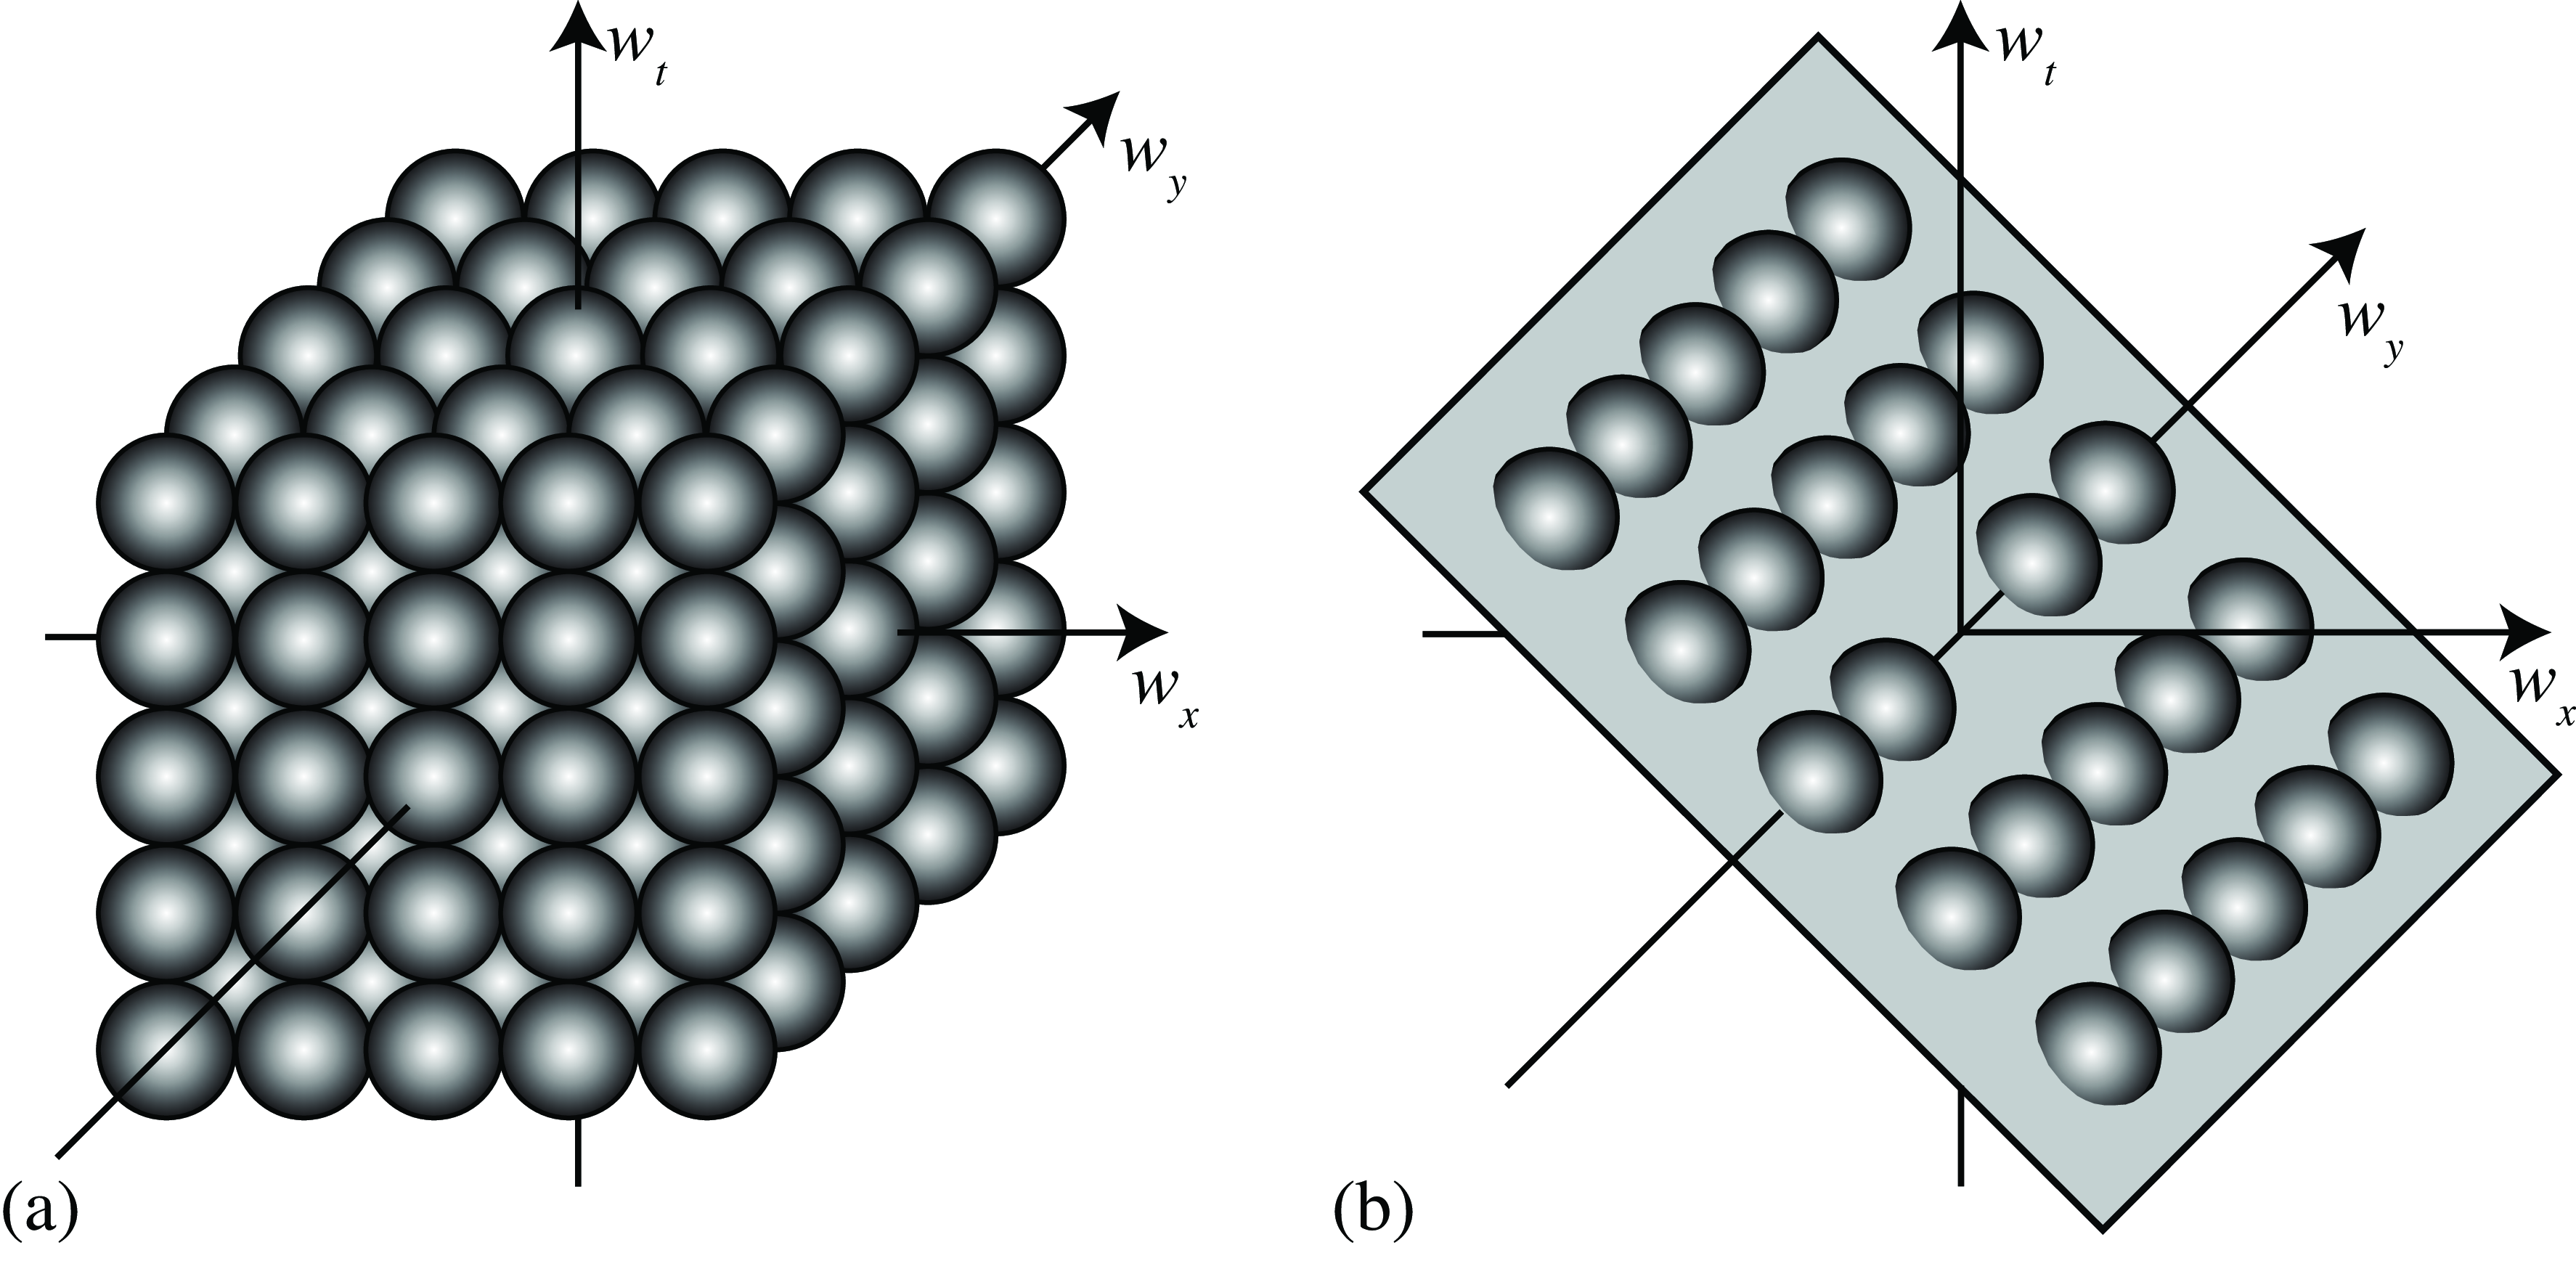
\includegraphics[width=1\linewidth]{figures/temporal_filters/gabor_spacetime_tiles.eps}
	}
	\caption{(a) Space-time Gabor filters tiling the full spatiotemporal frequency domain. (b) Subset of the Gabor filters selective to a particular velocity.}
	\label{fig:spacetimetiles2}
\end{figure}


As an illustration, \fig{\ref{fig:MT_velocity_tuned}} shows one possible architecture to create velocity-selective units.
The first layer is composed by space-time Gabor filters (cosine and sine), which are frequency-selective units. Here we represent the impulse response of each filter by a small $x-y-t$ cube. For each quadrature pair we compute the amplitude. Then amplitude outputs are combined according to form different planes in the Fourier domain to create velocity-selective outputs. A normalization layer can be added to normalize the outputs by dividing every output by the sum of all the amplitudes (not shown). The full architecture is nonlinear.

%The first layer is composed by Gabor filters (cosine and sine) which are frequency-selective units. The outputs of gabor filters are combined according to different planes in the Fourier domain to create velocity-selective outputs. 

Given an input sequence, one can estimate velocity by looking at the velocity-tuned unit with the strongest response.

\begin{figure}[t]
	\centerline{
		\includegraphics[width=1\linewidth]{figures/temporal_filters/MT_velocity_tuned.eps}
	}
	\caption{Architecture to create velocity-selective units. In the first layer, cosine and sine filters are combined to create phase invariant frequency-tuned outputs. In the second layer, the outputs of spatiotemporal Gabor filters are grouped according to different planes in the Fourier domain to create velocity-selective outputs. }
	\label{fig:MT_velocity_tuned}
\end{figure}







\section{Concluding Remarks}

In this chapter we have seen the power of using filter banks with some simple nonlinearities.

Hand-crafted filter banks started as a model of low-level vision mechanisms in humans, and became the basis to perform many visual tasks such as texture analysis \cite{RG:Heeger-Bergen95}, image segmentation \cite{Perona91}, motion analysis \cite{Heeger92}, orientation analysis \cite{Freeman90c}, image denoising \cite{Simoncelli96}, and many others.

These approaches had an advantage in that they were based on first principles and required no training data. However, note that performances when using hand-crafted architectures were limited. Many of the architectures we described in this chapter can be seen as precursors to many of the learning-based architectures we will discuss in subsequent chapters.

Before we dive into learning-based architectures, we will study multiscale image pyramids in the following chapter.
%In the next chapter we will study image pyramids.


